\documentclass[report.tex]{subfiles}
\begin{document}

This first chapter of the thesis motivates and defines
a \gls{DSL} for the modelling of general \gls{NN}s.
The first part of the chapter presents the theory behind second and third
generation \gls{NN}s, so as to posit requirements for the language. 
Finally this chapter will present the \gls{DSL} \index{Volr},
as a means to translate cognitive concepts into computational \gls{NN}
models.

\section{Neural networks}
\Gls{NN}s is a broad term that originates in the neuronal models from
biological brain \cite{Dayan2001}.
The general architecture of neural systems can be explained as circuits
of neurons \index{neuron} connected through weighted edges.
\cite{Russel2007, Dayan2001}.
In this abstract sense a neuron is defined as a computational unit that
takes a number of signals (inputs) and processes them through some
function $f$ that outputs a single value \cite{Eliasmith2004}.
From that perspective neural networks simply \textit{computes} an 
output based on some input why neural networks can be understood as
complex non-linear computations \cite{Eliasmith2004, Dayan2001}.

In a more concrete sense neural networks computes over either
continuous (e. g. voltage and numbers) or discrete signal, and they
can be modelled with or without a temporal dimension
\cite{Eliasmith2004, Russel2007, Schmidhuber2014}.

Common for many of the models are that they enrich the
input signals ($x$) with a weight as shown in \ref{eq:weightedsum}
\cite{Schmidhuber2014, Russel2007}. 
Given $n$ input neurons, the weighted sum is the value of each
input neuron scaled by a weight for that individual neuron.
Weights allow the model to adapt the relative importance of each
input neuron by modifying their weights, thus allowing the
model to \textit{train} to a given domain \cite{Schmidhuber2014, Russel2007}.

\begin{equation} \label{eq:weightedsum}
u = w \cdot x = \sum_{i=1}^n w_i x_i
\end{equation}

Discrete models without a temporal dimension were the foundation for
the first generation of neural networks \cite{Russel2007, Maass1997}.
They are based on the perceptron model as seen in equation
\ref{eq:perceptron}, also known as the McCulluch-Pitts neuron model
\cite{Eliasmith2004}.

\begin{equation} \label{eq:perceptron}
f(x) = \begin{cases}
	 1 & \text{if } u > 0\\
	 0 & \text{otherwise}
       \end{cases}
\end{equation}

\subsection{Second generation neural networks}
Second generation neural networks augment the perceptron model by
a) allowing continuous output values of a neuron and b) parameterising
the computation of the neuron by adding an \textit{activation function}
\index{activation function} for when the output ``activates'' 
\cite{Maass1997}.
\textit{Sigmoidal} functions are commonly used for activation functions
because they resemble the perceptron step function while 
retatining continuity (see figure \ref{fig:sigmoid})
\cite{Maass1997}.

\begin{figure}
\centering
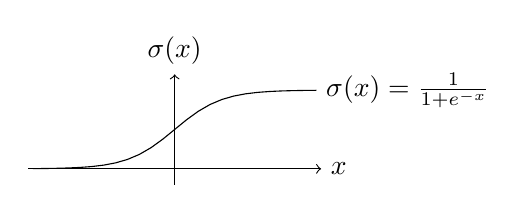
\begin{tikzpicture}[domain=-6:6,xscale=0.3]
  \draw[->] (-6.2,0) -- (6.2,0) node[right] {$x$};
  \draw[->] (0,-0.2) -- (0,1.2) node[above] {$\sigma(x)$};
  \draw plot (\x,{1 / (1 + exp(-\x))}) node[right] {$\sigma(x) = {1 \over 1 + e^{-x}}$};
\end{tikzpicture}
\caption{A sigmoidal (soft step) function.}
\label{fig:sigmoid}
\end{figure}

A number of variations for sigmoidal activation functions exist such as $tanh$ and
the rectified linear unit \index{ReLU} (ReLU, see equation \ref{eq:ReLU}). 
They are applied either in a feedforward or recurrent (cyclic) manor, where
the recurrent variant are forced to cope with temporal transformations to
terminate\footnote{It is possible to \textit{unfold} recurrent
networks to resemble the circular processes until a certain point, achieving
a similar effect to temporal signal transformation, see \cite{Mozer1995}.}
\cite{Schmidhuber2014}.

\begin{equation} \label{eq:ReLU}
f(x) = \begin{cases}
         0 & \text{if } x < 0 \\
	 x & \text{otherwise}
       \end{cases}
\end{equation}

\subsection{Third generation neural networks}
Constructing a network of neuron models essentially creates a non-linear
response to a given numerical vector \cite{Russel2007}.
This transformative view can be adopted to biological \gls{NN}, where
the data being transferred are no longer vectors, but discrete
\textit{spikes} of electrical current \cite[p. 32]{Dayan2001, Eliasmith2004}.
In this case the activation of a spike can be understood as a function
of the electric current to the neuron cell along with the cell weights,
similar to the weighted sum in equation \ref{eq:weightedsum}
\cite[p. 234]{Dayan2001}.

There is a temporal dimension to this because signals in biological 
networks arrive from multiple sources in parallel \cite{Eliasmith2004}.
Lapicque presented the first model of conductance over time in 1907,
dubbed the \texit{integrate-and-fire} model, because neurons essentially
integrate received current over time to determine whether they should fire 
\cite{Dayan2001, Eliasmith2004}.
This understanding is the foundation for the \textit{third} generation
neural networks, where the computations occur in spikes over time 
\cite{Maass1997}.
Lapicque's model has been elaborated in the \texit{leaky
integrate-and-fire} model, which introduces a numerical ``leak''
into the model, that acts as a \textit{weight} for the neuron integration
\cite{Eliasmith2004, Eliasmith2015}.

\subsubsection{Encoding and decoding in spiking neural networks}
To align the bitwise numerical representation with the neural spikes
it is necessary to encode and decode the signals.
Because of the temporal nature of spiking neural networks, probability
distributions are commonly used to describe 
Given a current for background firing rates
Assuming there are $n$ inputs to a neuron with $i$ bits of information,
an encoder kk


An example of a network is shown in 

\begin{figure}
\centering
\begin{tikzpicture}{x=1.5cm, y=1.5cm}
  \foreach \m/\l [count=\y] in {1, 2, 3}
    \node [every neuron/.try, neuron\m/.try] (input-\m) at (0,2.5-\y) {};
\end{tikzpicture}
\caption{An example neural network with a single hidden layer.}
\label{fig:nn-example}
\end{figure}

circuits of computational
units connected through weighted edges \cite{Dayan2001, Eliasmith2004}.

% TODO: Distributions of properties instead of actual properties

% Both types of network are architecturally similar, and both are conceived from
% the same physiological principles \autocite{dayan2001, russel2007, Nilsson2009, schmidhuber2014}.
% The implementations, however, vary greatly.

% To ensure internal and external validity in and between the two network types,
% it is desirable that the models are as closely related from a theoretical and
% practical perspective as possible.
% Additionally, to test the hypothesis, it is required that both the artificial
% and spiking models can be simulated on regular machine architecture, while
% the spiking model requires a neuromorphic hardware platform.

% An optimal approach would be to find a tool that leverages the similarities
% of the network types, while integrating with the diverse simulated or emulated
% targets.
% That is, an abstract model of neural networks that can translate into
% heterogeneous back-ends, while retaining a high degree of inter-model validity.

% A number of general frameworks for artificial neural networks
% exist\footnote{
%   Among others, see \autocite{ONNX2018}, \autocite{PyTorch2018}, \autocite{TensorFlow2018},
%   \autocite{Keras2018} and DyNet \autocite{Neubig2017}.
% }, but none of them extend to the spiking domain.
% Conversely a number of choices exist for neuromorphic modelling\footnote{
%   %TODO: Find sources on internal IBM/Intel stuff
% }, but they exclusively evaluate to neuromorphic or spiking neural network
% backends \autocite{Jordan2018}.

\subsection{Learning in neural networks}

\subsubsection{Backpropagation}

\section{DSL requirements}

\section{Similar work}

This sections presents the \gls{DSL} Volr. \index{Volr}
The main purpose of Volr is to define clear and reproducible
experiments whose semantics are retained regardless of
the runtime environment.
The specification in its current form is relatively simple, but sufficiently 
complicated for the purpose of this thesis.
It focuses solely on the topology of networks, thus
separating the network description from any generation-specific properties
of neurons or neuron populations.

The first requirement is achieved through an unambiguous syntax inspired
by the lamdba calculus \cite{Pierce2002}.
Figure \ref{fig:volr-expr} shows the BNF notation for expressions, values and types
in Volr. 
Figure \ref{fig:volr-rules} lists evaluation rules for the correct
interpretation of the expressions.

% Expression figure
\begin{figure}
  \begin{tabular}[t]{l l}
    expressions & \texttt{$e$ ::= $n$} \\
    & \begin{minipage}{0.6\textwidth}
      \begin{Verbatim}[mathescape,commandchars=\\\{\}]
    | \textbf{dense} $n\ m$
    | \textbf{let} $x = e$ \textbf{in} $e'$
    | $e\ \obar\ e'$
    | $e\ \ominus\ e'$
    | $\neg e$
      \end{Verbatim} 
      \end{minipage} \\

    & \\ % Empty space 

    values
    & \texttt{$v$ ::= $\textbf{net}\ n\ m$} \\
    
    & \\ % Empty space
    types
    & \texttt{$\tau$ ::= \textbf{int} | \textbf{net} $n\ m$} \\
  \end{tabular}

  \caption{Expressions, values and types of the Volr language.}
  \label{fig:volr-expr}
\end{figure}
\begin{figure}
\begin{prooftree}
  \AxiomC{}
  \UnaryInfC{$\Gamma \vdash n : \mathbf{int}$}
\end{prooftree}
\begin{prooftree}
  \AxiomC{}
  \UnaryInfC{$\Gamma \vdash \mathbf{stim}\ n : \mathbf{layer}\ n$}
\end{prooftree}
\begin{prooftree}
  \AxiomC{}
  \UnaryInfC{$\Gamma \vdash \mathbf{pop}\ n : \mathbf{layer}\ n$}
\end{prooftree}
\begin{prooftree}
  \AxiomC{$\Gamma (x) = \tau$}
  \UnaryInfC{$\Gamma \vdash x : \tau$}
\end{prooftree}
\begin{prooftree}
  \AxiomC{$\Gamma \vdash e_1 : \mathbf{layer}\ n$}
  \AxiomC{$\Gamma \vdash e_2 : \mathbf{layer}\ m$}
  \AxiomC{$\Gamma \vdash w : \mathbf{float}$}
  \TrinaryInfC{$\Gamma \vdash \otimes\ e_1\ e_2\ w : \mathbf{con}\ n\ m$}
\end{prooftree}
\begin{prooftree}
  \AxiomC{$\Gamma \vdash e_1 : \mathbf{layer}\ n$}
  \AxiomC{$\Gamma \vdash e_2 : \mathbf{layer}\ m$}
  \AxiomC{$\Gamma \vdash w : \mathbf{float}$}
  \TrinaryInfC{$\Gamma \vdash \ominus\ e_1\ e_2\ w : \mathbf{con}\ n\ m$}
\end{prooftree}
\begin{prooftree}
  \AxiomC{$\Gamma \vdash e : \tau$}
  \AxiomC{$\Gamma [v : \tau] \vdash e' : \tau$}
  \BinaryInfC{$\Gamma \vdash \mathbf{let}\ x = e\ in\ e' : \tau$}
\end{prooftree}

  \caption{Evaluation rules in Volr.}
  \label{fig:volr-rules}
\end{figure}



The constant expression $n$ is simply an integer that evaluates to the type 
\texttt{\textbf{int}} ($e1$). 
Similarly to the lambda calculus, the \texttt{\textbf{let}} binding binds
the string constant $x$ to the expression $e$ in an encapsulated
environment $e'$ \cite{Pierce2002}.
That constant can later be referenced in the $e'$ expression 
through the string $x$ as shown in $e2$.

The \texttt{\textbf{dense}} expression describes a network of two
populations, and is the most basic concept in the \gls{DSL}.
Notice the distinction between a neural network \textit{layer}
such as \texttt{\textbf{dense}} and a population. 
In a \texttt{\textbf{dense}} network layer, every neuron from the
first population is connected to every neuron in the second population
(\textit{densely} or all-to-all).
The two parameters $n$ and $m$ defines the number of neurons in the first and 
second layer respectively, and evaluates to the \texttt{\textbf{net}}
fundamental network type and value, as shown in $e3$. 
Considering how each neuron is a type of classifier, these numbers
illustrate the \textit{dimensionality} of the network, such that the number of
dimensions in the input is truncated (or expanded) to classify the
dimensionality of the output layer.

The $\obar$ (sequential) operator binds two networks sequentially,
such that the output layer of the first network becomes the input layer 
of the second network.
The two networks $e$ and $e'$ will share one of the neuron populations, why
the output size of the first layer is required to be equal to the input
size of the second layer ($e4$).

The $\ominus$ (parallel) operator parallelises two networks by duplicating
the input from the previous layer and merging the outputs into a single
layer ($e5$).
The input feeds into both $e$ and $e'$, such that the input dimension of
the network must be shared by the two layers ($l$). 
The output from the network is stacked such that each neuron from each
population corresponds to one output neuron ($e_{out} + e'_{out}$).
This is done to preserve the meaning of each parallel population.

Taken together these constructs can express simple neural networks and
the properties of their connections. 
Figure \ref{fig:volr-examples} shows a number of example networks
that visualises four examples of networks. 

\begin{figure}
  \ContinuedFloat*
  \begin{tabular}[t]{c c}
    \begin{minipage}{0.5\textwidth}
      \begin{Verbatim}[mathescape,commandchars=\\\{\}]
\textbf{let} s = stim 2 \textbf{in}
  \textbf{let} p = pop 2 1 \textbf{in}
    s $\otimes$ p
      \end{Verbatim}
    \end{minipage} & \begin{minipage}{0.5\textwidth}
      \includegraphics[width=\textwidth]{chapters/volr/example1.pdf}
    \end{minipage}

  \end{tabular}
  \caption{A textual and visual example of a network with a stimulus,
    a population and an implicit output.}
  \label{fig:volr-example1}
\end{figure}

\begin{figure}
  \ContinuedFloat*
  \begin{tabular}[t]{c c}
    \begin{minipage}{0.5\textwidth}
      \begin{Verbatim}[mathescape,commandchars=\\\{\}]
\textbf{let} s = stim 2 \textbf{in}
  \textbf{let} p = pop 2 1 \textbf{in}
    s $\otimes$ p
      \end{Verbatim}
    \end{minipage} & \begin{minipage}{0.5\textwidth}
      Hello
    \end{minipage}
  \end{tabular}
\label{fig:volr-examples}
\end{figure}

\FloatBarrier

\end{document}
